\subsection{Replicação}

A fórmula para encontrar o servidor em que está localizado um objecto com um dado uid é: \textit{hash(uid) mod (número de servidores)}. Para encontrar o servidor com o objecto primário a função de dispersão retorna o uid, para encontrar o servidor com a réplica a função de dispersão retorna uid + (número de objectos por bloco).

O \textit{master} contém as fórmulas mais recentes e tanto os servidores como os clientes guardam estas fórmulas em \textit{cache} no primeiro pedido efectuado ao master, para evitar pedidos remotos desnecessários.

Os clientes podem aceder aos dados de 2 maneiras:

\begin{itemize}
\item \textbf{Com replicação:} 

\begin{enumerate}
\item Cada leitura é efectuada ao servidor primário do objecto, e caso este não esteja disponível o valor é obtido do servidor secundário.

\item Cada escrita é efectuada no primário e no secundário, mas o cliente não espera pelas respostas. Caso existam mais de 2 réplicas, o cliente envia no máximo a 5 servidores que replicam para os restantes.
\end{enumerate}

\begin{figure}
\centering
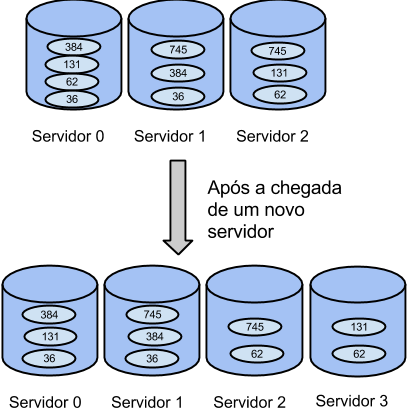
\includegraphics[width=0.4\textwidth]{migracao.png}
\caption{\label{fig:migracao}Migração dos dados face à entrada de um novo servidor.}
\end{figure}

\item \textbf{Sem replicação:}

\begin{enumerate}
\item Cada leitura é efectuada apenas no servidor responsável por guardar aquele objecto, se o servidor estiver em baixo a transacção é abortada.

\item Cada escrita é efectuada apenas no servidor responsável por guardar aquele objecto, se o servidor estiver em baixo a transacção é abortada.
\end{enumerate}
\end{itemize}